

\section{ Gradient descent 's algorithm }
\subsection{Introduction}

Gradient descent is a general technique for minimizing  twice-differentiable functions through its slope. \cite{LFD}
It is used to find local minimums. The start point is crucial in the search.  

The basic idea is to update the weights using the gradients until it is not possible to continuous minimizing the error.


\medskip

\subsection{Math}

In order to understand the algorithm we are going to define: 

Let $w(0) \in \mathbb{R}^d$ be an arbitrary initial point,
$E : \mathbb{R}^d \times \mathbb{R}^d \longrightarrow \mathbb R$
a class $C^1$ function. The learning rate or step size $\eta \in \mathbb{R}^+$
is a experimental coefficient about how much are we going to follow the slope to obtain the new weight.  
Let  $w(t) \in \mathbb{R}^d  \quad t \in \mathbb N$ be the weight for $t$ iteration which is defined as

\begin{equation*}
  w(t+1) = w(t) - \eta \nabla E_{in}(w(t))
\end{equation*}

\subsubsection{ Properties}

\begin{itemize}
\item This algorithm gives local minimums.
\item Convergence it is not assured, so it would be necessary some stop criteria. 
\item For a convex function it would be a unique global minimum.
\item The learning rate $\eta$ variable in time  is important: fixes learning gradient descent algorithm. 
\end{itemize}


\subsection{Algorithm}

The following code snippet implement the algorithm, where $w(0)$ is the $initial\_point$, $E$ is the error, $\nabla E_{in}(w)$ is $gradient\_function$ and
finally $\eta$ is $eta.$ The value $\eta = 0.1$ is a heuristic basic on purely practical observation \cite{LFD}.


In order to avoid an infinite search, our stop criteria are a limit in the number of iterations $max\_sitter$ and an error tolerance. 

\begin{minted}{python} 

  def gradient_descent(initial_point, loss_function,
                gradient_function,  eta, max_iter, target_error):
    '''
    initicial point: w_0 
    E: error function 
    gradient_function
    eta:  step size 

    ### stop conditions ###
    max_iter
    target_error

    #### return ####
    (w,iterations)
    w: the coordenates that minimize E
    it: the numbers of iterations needed to obtain w
    
    '''

    iterations = 0
    error = E( initial_point[0], initial_point[1])
    w = initial_point
  
    while ( (iterations < max_iter) and(error > target_error)): 

        w = w - eta * gradient_function(w[0], w[1])
        
        iterations += 1
        error = loss_function(w[0], w[1])
 
    
    return w, iterations
        
\end{minted}

\subsection{Problem 1}

We want to solve the following problem: %\\

Use gradient descent's algorithm to find a minimum for the
function


\[E(u,v) = (u^3 e^{(v-2)} - 2* v^2 e^{-u})^2.\]

Set $(u,v)=(1,1)$ as initial point and use learning rate $\eta = 0.1$.

\subsubsection{Compute analytically the gradient of $E(u,v)$}


\begin{multline*}
  \nabla E(u,v) = \left( \frac{\partial}{\partial u}(u^3 e^{(v-2)} - 2* v^2 e^{-u})^2 , \frac{\partial}{\partial v} (u^3 e^{(v-2)} - 2 v^2 e^{-u})^2 \right) = \\
 =  \left(2(u^3 e^{(v-2)} - 2* v^2 e^{-u})(3u^2e^{(v-2)} + 2 v^2 e^{-u} ), 2(u^3 e^{(v-2)} - 2* v^2 e^{-u})(u^3 e^{(v-2)} - 4 v e^{-u}) \right)
\end{multline*}


\subsubsection{Number of iterations and final coordinates.}

Firstable we need to use 64-bits float, so we are going to use the data type $float64$ of numpy library \cite{float64}.

The functions' declaration are:

\begin{minted}{python}
  def dEu(u,v):
    '''
    Partial derivate of E with respect to the variable u
    '''
    return np.float64(
        2
        *( 3* u**2 * np.e**(v-2) + 2*v**2 * np.e**(-u) )
        *( u**3 * np.e**(v-2) - 2*v**2 * np.e**(-u))
    )
    
def dEv(u,v):
    '''
    Partial derivate of E with respect to the variable v
    '''
    return np.float64(
        2*
        ( u**3 * np.e**(v-2) - 2*v**2 * np.e**(-u) )
        *( u**3 * np.e**(v-2) - 4*v * np.e**(-u))
    )


def gradE(u,v):
    ''' 
        gradient of E
    '''
    return np.array([dEu(u,v), dEv(u,v)])

\end{minted}

To obtain the number of iterations and the final coordinates, the only thing we need to do is to call $gradien\_descent$ function with the initial conditions:

\begin{minted}{python}
eta = 0.01 
max_iter = 10000000000
target_error = 1e-14
initial_point = np.array([1.0,1.0])
w, it = gradient_descent( initial_point,
                          E,
                          gradE,
                          eta,
                          max_iter,
                          target_error )
\end{minted}

The result are:

\begin{itemize}
\item Numbers of iterations: $178.$
\item Final coordinates: $( 1.162 ,  0.924 ).$
\end{itemize}

A 3d graph with the result is 

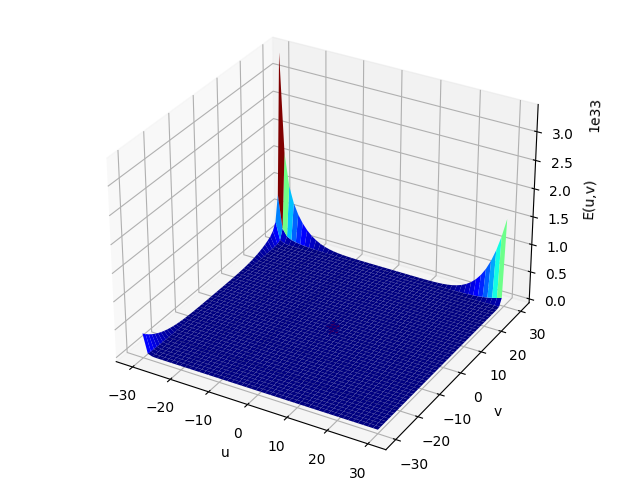
\includegraphics[width=\linewidth]{1_graph.png}



\subsection{Problem 2}


For function $f(x,y) = (x+2)^2 + 2(y-2)^2 + 2 \sin (2 \pi x) \sin (2 \pi y)$

\subsubsection{ Use gradient descent to minimize $f$}

The initial point is $(x_0 = -1, y_0 = 1)$,
learning rate is $\eta = 0.01$ and the maximum number of iterations must
be $50$.  Plot the result and repeat the experiment with  $\eta = 0.1$. 

Firstly we are going to calculate partial derivatives and gradient of $f$.

\begin{equation*}
  \frac{\partial }{\partial x} f = 2 (x + 2) + 2 \sin (2 \pi y) \cos ( 2 \pi x) 2 \pi =  2 (x + 2) +  4 \pi \sin (2 \pi y) \cos ( 2 \pi x)   
\end{equation*}

\begin{equation*}
  \frac{\partial }{\partial y} f = 2 (y - 2) +  4 \pi \sin (2 \pi x) \cos ( 2 \pi y)   
\end{equation*}


It is important to realise that $f(x,y) <0$ for some values in $\mathbb R^3$ so the error target has been omitted in this algorithm.   


Now the new algorithm is
\begin{minted}{python}
  def gradient_descent_trace(initial_point, loss_function,
    gradient_function,  eta, max_iter):
    '''
    initicial point: w_0 
    loss_function: error function 
    gradient_function
    eta:  step size 

    ### stop conditions ###
    max_iter

    #### return ####
    (w,iterations)
    w: the coordenates that minimize loss_function
    it: the numbers of iterations needed to obtain w
    
    '''

    iterations = 0
    error = loss_function( initial_point[0], initial_point[1])
    w = [initial_point]
  
    while iterations < max_iter: 

        new_w = w[-1] - eta * gradient_function(w[-1][0], w[-1][1])
        
        
        iterations += 1
        error = loss_function(new_w[0], new_w[1])
        w.append( new_w ) 
    
    return w, iterations
  
  \end{minted}


  After 50 iterations for  $\eta = 0.01$, the  final coordinates are $(-1.269, 1.287)$ and their value is $-0.381$. The graph, which shows the relation between iterations and the function minimization is


  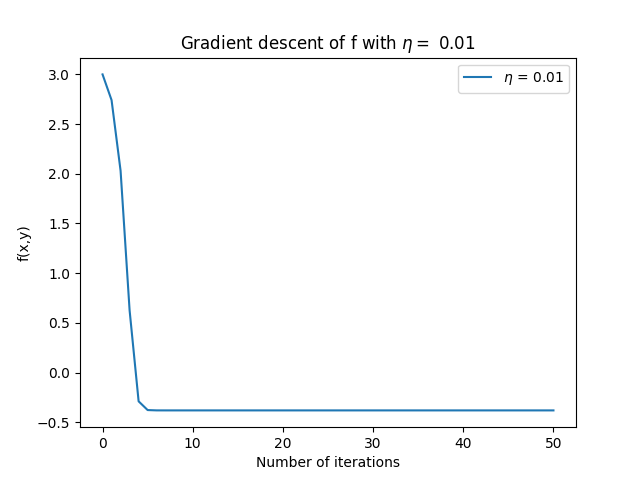
\includegraphics[width=\linewidth]{1_3_smaller_eta}

  As far as we have seen, before the $10^{th}$ iteration we are really close to  the minimum and stay there without fluctuate.

  On the other hand, after 50 iterations for  $\eta = 0.1$ the final coordinates are $(-2.939, 1.608)$ and their value is $0.724$, so as we can see this result is worse than the last one.

  In the following graph we can see the evolution fluctuation of the images iteration by iteration 

  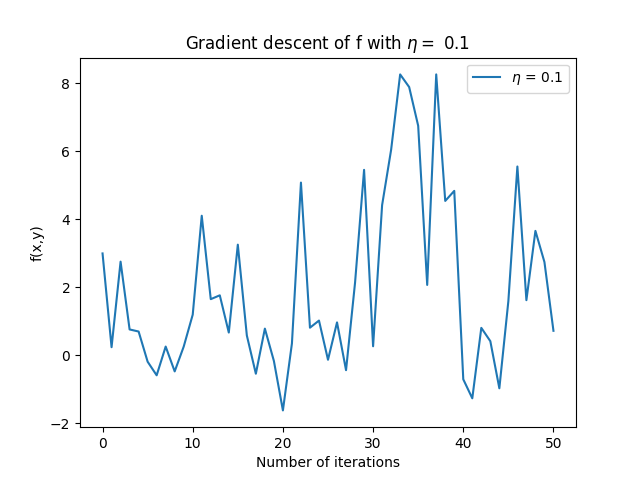
\includegraphics[width=\linewidth]{1_3_bigger_eta}.

 The reason for this irregularity  is that the step size is too big, so it skips the minimum.

 We can also  compare the two experiment in the following graph.
 
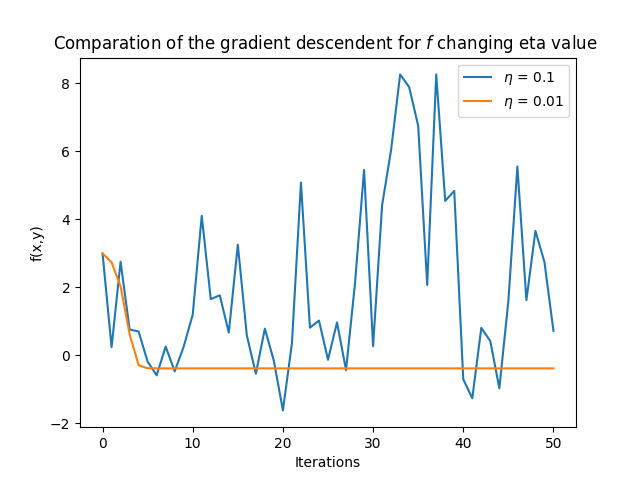
\includegraphics[width=\linewidth]{1_3_comparation_eta}.


    Moreover, basic on its mathematics proof, which use Taylor's series, we know that it should be small, but if it is too small the algorithm will never reach the minimum in a right time.

 Let see a new example, now $\eta = 10^{-14}$, after 50 iteration  the final coordinates are $(-1, 1)$  and the value is $3$, so this new selection is even worse that the one with the bigger step size, although it goes without oscillate.  

 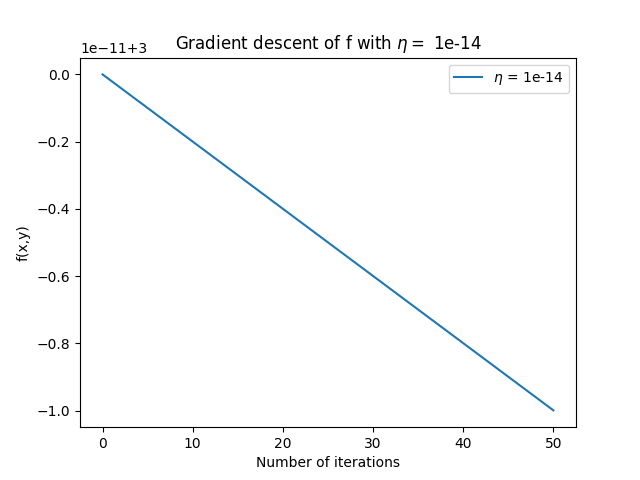
\includegraphics[width=\linewidth]{1_3_epsilon_eta}
 
 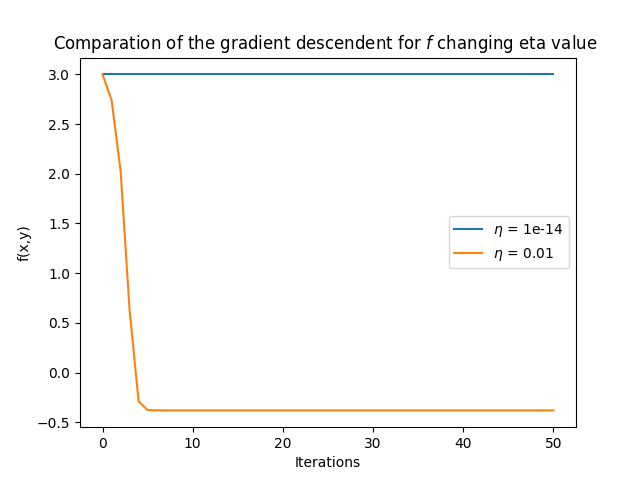
\includegraphics[width=\linewidth]{1_3_eta_and_smaller.png}
 
  As a conclusion, a priory, it is difficult to select a step size value, each problem should have an appropriate one, and the selection must be empirical. Even though some heuristic \cite{LFD} tell that $\eta = 0.01$ its a good try.  

 
  

\subsubsection{Minimum value }


Before running the algorithm is important to think about a good value for the learning rate $\eta$. Based on the last section $\eta = 0.1$ is a good one. 


After run the program the  results are

\begin{center}
  \begin{tabular}{ |c|c|c| }
    \hline
    Initial point  & Final coordinates & Final value  \\ 
    \hline

    (-0.5 -0.5) &  (-0.793 -0.126) &   9.125 \\
(1 1) &  (0.677 1.29) &   6.437 \\
( 2.1 -2.1) &  ( 0.149 -0.096 ) &   12.491 \\
(-3  3) &  (-2.7315  2.713) &  -0.381 \\
(-2  2) &  (-2.  2.) &  0 \\
    
 
 \hline
\end{tabular}
\end{center}


This example gives the idea that the local minimums found depend on the start point and a priory, unless we know some properties
of the function such as convexity or monotony we are not able to assure that the minimum found is global.

For a mathematical study we need differentiable functions, and a technique to  find where their zeros are, so we need to solve their equations. Some time
this is not possible and we use numeric methods.




\subsection{ Final conclusion about finding global functions' minimum}  


- Properties differentiable, arbitrary initial point, eta, computational cost...  TO-DO


